%\documentclass[journal]{new-aiaa}
\documentclass[conf]{new-aiaa} %for conference papers
\usepackage[utf8]{inputenc}

\usepackage{graphicx}
\usepackage{subcaption}
\usepackage{amsmath}
\usepackage[version=4]{mhchem}
\usepackage{siunitx}
\usepackage{longtable,tabularx}
\usepackage{gensymb}
\setlength\LTleft{0pt} 

\title{Towards an Aircraft with Reduced Lateral Static Stability Using Electric Differential Thrust}

\author{Eric Nguyen Van\footnote{PhD, eric.nguyen-van@isae.fr, eric.nguyen\_van@onera.fr}}
\affil{ISAE DCAS, Toulouse, France}
\affil{ONERA DTIS, Toulouse France}
\author{Daniel Alazard\footnote{Professor Researcher, daniel.alazard@isae.fr.} and Philippe Pastor\footnote{Professor Researcher, philippe.pastor@isae.fr.}}
\affil{ISAE DCAS, Toulouse, France}
\author{Carsten D\"oll\footnote{Research engineer, carsten.doll@onera.fr.}}
\affil{ONERA DTIS, Toulouse, France}
%
%\author{Eric Nguyen Van\footnote{PhD candidate, ISAE-ONERA}, second author\footnote{blablabla}}.
%\affil{ISAE-ONERA, Toulouse, France}
%\author{Philippe Pastor\footnote{Enseignant Chercheur, DCAS, philippe.pastor@isae.fr.} Daniel Alazard\footnote{Enseignant Chercheur, DCAS, daniel.alazard@isae.fr.}}
%\affil{ISAE-SUPAERO, Toulouse, France}
%\author{Carsten D\"\o ll \footnote{Research Engineer, DTIS, carsten.doll@onera.fr.}}
%\affil{ONERA, Toulouse, France}

%Title : "Towards an Aircraft with Reduced Static Stability using Electric Differential Thrust"
%
%Introduction :
%	Reduction of surface drag by reduction of stability surfaces
%	Problematic with the VT dimensioning
%	New technology : DEP
%	Study the possibilities of VT reduction by comparison of flight envelop
%Math modeling
%	Equation of flight
%	Modeling differential thrust
%	Solving the problem by optimization
%Parametric Aerodynamic Database
%	Panel/VLM analysis of ATR72 with and without VT
%	Introduction of Nicolossi's method to predict VT lift coefficient and correction of lateral coefficients
%Results (study of single/multiple engine failure at take off)
%	Baseline ATR72 (twin engine) with different VT size
%	DEP configuration of the Baseline with different VT size
%	Effect of varying the number of engine, ratio of inoperative engine and total on-board power
%Conclusion
%	Sum up results
%	Why differential propulsion is interesting to reduce VT
%	Implication and future work

\begin{document}

\maketitle

\begin{abstract}
In the context of aircraft drag reduction, we study the possibility of reducing the area of the vertical tail using Distributed Electric Propulsion while maintaining lateral stability with active Differential Thrust. Distributed Electric Propulsion is usually thought of as a mean to increase aerodynamic efficiency by exploiting the benefic effects of accelerating air around key parts of the aircraft. However, it can also be seen as a collection of actuation devices generating additional moments through Differential Thrust. When the engine are distributed along the lateral axis, the aircraft designer may take advantage of the increase of control authority on yaw to reduce the static stability or the control authority provided by the vertical tail. This in turn would allow a reduction of vertical tail surface area. In order to explore and assess this idea, we suggest a framework to compare flight qualities of a traditional configuration versus a configuration using Distributed Electric Propulsion and Differential Thrust. It provides information on the flight envelop and stability of the aircraft by computing a map of the equilibriums. Thanks to a global approach, it allows to study any aircraft or DEP configurations in any flight phase. In addition, a key feature of the framework is the inclusion of the VeDSC method to compute analytically the contribution of the vertical tail to lateral stability. Here are presented the first results and potential of using differential thrust to reduce the area of the vertical tail and the reasons for us to continue developing this framework.
\end{abstract}

\clearpage

\section*{Nomenclature}

%\noindent(Nomenclature)

{\renewcommand\arraystretch{1.0}
\noindent\begin{longtable*}{@{}l @{\quad=\quad} l@{}}
CCV & Control Configured Vehicle\\
MDO & Multi-Disciplinary Optimization\\
DEP & Distributed Electric Propulsion\\
VT & Vertical Tail\\
AR & Aspect Ratio\\
$\rho$ & Air density (Kg/m$^3$)\\
$V$ & Speed (m/s)\\
$V_s$ & Stall speed (m/s)\\
$V_{MC}$ & Minimum control speed (m/s)\\
$P$ & Power (W)\\
$T$ & Thrust (N)\\
$\eta$ & Efficiency (-)\\
$S$ & Wing surface area (m$^2$)\\
$S_v$ & Vertical Tail surface area (m$^2$)\\
b & Wingspan (m)\\
$l_F$ & VT longitudinal position with respect to wing aerodynamic center (m)\\
$z_v$ & vertical position of the mean aerodynamic chord of the VT (m)\\
$V_v$ & VT volume (-)\\
$y$ & Lateral position of engine (m)\\
$m$ & Mass (Kg)\\
$g$ & Gravitational acceleration (m.s$^{-2}$)\\
$\beta$ & Side slipe angle ($\SIUnitSymbolDegree$)\\
$\phi$ & Bank angle ($\SIUnitSymbolDegree$)\\
$\gamma$ & Climb angle ($\SIUnitSymbolDegree$)\\
$\mu$ & Aerodynamic bank angle ($\SIUnitSymbolDegree$)\\
$\Omega$ & Turning rate (rad.s$^{-1}$)\\
$\delta_a$ & Aileron input ($\SIUnitSymbolDegree$)\\
$\delta_R$ & Rudder input ($\SIUnitSymbolDegree$)\\
$\delta_m$ & Throttle level (-)\\
$C_D$ & Drag force coefficient (-)\\
$C_{Y}$ & Lateral force coefficient (-)\\
$C_L$ & Lift force coefficient (-)\\
$C_l$ & Rolling moment coefficient (-)\\
$C_m$ & Pitch moment coefficient (-)\\
$C_n$ & Yawing moment coefficient (-)\\
$a_v$ & VT lift slope coefficient (-)\\
\multicolumn{2}{@{}l}{Subscripts}\\
v & Vertical Tail\\
0 & Nominal condition or sea level\\
b & Body attached frame\\
\end{longtable*}}


 \section{Introduction}
\lettrine{R}{educing} static stability of aircrafts is a way to increase flight performances in terms of manoeuvrability and drag reduction. The first case benefits fighter aircrafts which are usually designed unstable by manipulating stability surfaces and position of the center of gravity. When reducing the tail volums i.e stability surfaces and the level arms, we also achieve a significant reduction in drag due to the diminution of wetted surfaces.In the civilian domain, this effect is increaslingly exploited due to the important flight performances increase \cite{HermanImpactControlConceptonDesign}, \cite{Abzug}.

To obtain a high level of performance improvement, the aircraft design strategy must be modified so as to include a stability and control block that can act on the geometry of the airplane. This way, the designer can take advantage of fly by wire and active control. This domain is called Control Configured Vehicle (CCV) and is not limited to airplane\cite{Abzug}. An example of aircraft design based on CCV principles has been describe by Anderson and Mason in \cite{Anderson_CCV_design}. The authors introduce the main problematic with CCV; the automatisation of control law design and flight quality assessment in order to embbed the discipline in a Multi-Disciplinary Optimization MDO . They propose a solution based on fuzzy logic to include CCV in an MDO. In the following years B. Chudoba and H. Smith \cite{Chudoba_generic_method} as well as R. E. Perez and H. T. Liu \cite{LiuPerezMDOFramework}, both presented an MDO framework designing stability and control laws based on Stability Augmentation System and pole placement technics with B. Chudoba focusing on generic modeling and characterisation. More recently a study from \cite{WelsteadConceptualDesignAugmentedStability} shows a methodology for inclusion of stability and control using optimal control into MDO while Y. Denieul \cite{YannDenieul} shows in his thesis the integrated optimization of actuation surfaces together with the control law based on $H_\infty$ methods. All these examples tend towards a more global approach in aircraft design due to the coupling of two or more disciplines, here flight stability and control, flight performances.

While methods exist for designing aircrafts with relaxed longitudinal stability \cite{CosenzaHandlingQualities}, the reduction of lateral static stability is bounded by stability requirements arising from emergency situations . The vertical stabilizer is dimensioned to handle single engine failure and/or strong lateral winds up to 25 kt \cite{FeuersangerReducedStability}, \cite{AFC_NASA_report_Mooney}, \cite{NicolosiInvestigationVertical}, \cite{CS25}, \cite{MorrisFlDynCstinMDO}. Usually the parameter constraining the size of the vertical stabilizer is the Minimum Control Speed : $V_{MC}$ definied by certification specifications as the minimum velocity at which, if an engine is made inoperative, the vertical tail has sufficient control authority to counter the yawing moment created by the remaining engine at maximum take off power within $5\SIUnitSymbolDegree$ of bank angle \cite{CS25}. This constraint is a hard limit for the reduction of the rudder, impacting the design for the whole Vertical Tail (VT). In addition as Morris suggests in \cite{MorrisFlDynCstinMDO}, the VT is often over-dimensioned to cope with non-linear viscous effects such as masking by the fuselage. A lack of adapted tool able to predict the performance of the VT in these conditions is called responsible for this case.
%for the reduction of the vertical tail because it must satify a static equilibrium.

Efforts for reducing the fin are taken both in research institutions and aircraft industry. They include better performance prediction for design phase \cite{dellavecchia} as well as flow control to increase fin efficiency \cite{InnovativeFlow_Lin}. In this last example, a possible reduction of the fin area could amount to 15\% with a total drag reduction of 0.9\%.

We envision to increase this reduction by using a new game changing technology that has recently gained interest among aircraft propulsion system; Distributed Electric Propulsion and differential thrust. Differential thrust is already used in current multi-engine aircrafts in case of complete loss of hydraulic system as a mean to control the aircraft. In this case, it is called Propulsion Controlled Aircraft \cite{TouchdownPCA}, a system developed first at NASA Dryden center. However, it cannot be used as a mean to increase lateral stability because of the lack of engine redundancy and of the large reaction time of turbomachines.

Recently, more and more interest has been held on electric airplanes. Though studies usually focus on the challenge of energy storing, we will focus and exploit the characteristics of electric engines. These ones are our actuators for differential thrust. The reader is refered to \cite{MisconceptionMoore} for a complete list of electric engine advantages. We will retain only the following; \emph{scale free efficiency} and \emph{high power density}. They allow to rethink the way of airframe propulsion integration. The designer can freely place the engines where they may increase aerodynamic performances. Two effects are usually seeked; \textbf{1.}Increase maximum lift by blowing and \textbf{2.}Bounday Layer Ingestion for drag reduction \cite{Assessment_of_DEP}, \cite{Turboelec_prop_analysis_nasa}. This is the case for the all electric concept plane AMPERE from ONERA \cite{Ampere_concept} where efans are integrated to the wing to benefit from blowing effects and NASA aircraft X57\cite{DesignPerfSceptor}. For this last example the distributed engines are expected to replace high lift devices.
The advantages for lateral control with differential thrust are threefold:
\begin{itemize}
	\item \textbf{Redundancy} : if one or more critical engines are suddenly made inoperative, only a small portion of the thrust is lost. There remain an important number of engine to reallocate the thrust.
	\item \textbf{Reaction time}: with small electric engines the reaction time can be of the order of $10^{-1}$s \cite{ActionneurElectric}, therefore fast with respect to aircraft flight dynamics.
	\item \textbf{Level-arm}: the engines being distributed along the wing (in the previously mentioned airplanes), we beneficiate from an important level arm without adding specific structures.
\end{itemize}

%We further assume no aerodynamic interaction effects between the wing and the propulsion system. This is outside the scope of the present study. We only assume point force of direction always parallel to the body x-axis as shown in Fig~\ref{fig:AmpereTop}.

Though the idea has been suggested in \cite{Turboelec_prop_analysis_nasa}, example and study of differential thrust for yaw control and relaxed lateral stability has, to the best of the authors knowledge, not yet received much attention. Hence, the goal of our study is to explore the possibilities of relaxing lateral stability by using differential thrust with electric propulsion and more specifically the requirements in terms of design.
%The final delivery would be a block of stability and control ready to be included into an MDO which allows the designer to optimize the size of the vertical stabilizer and conceive the propulsion system accordingly.

A detailled treatment of the distributed propulsion is not the approach retained for this study. Because electric propulsion is easily integrated into airframe, important synergies can exit between aerodynamics, structure, flight control and propulsion. This multiphysic environment necessitate a global approach to study DEP aircraft. %The authors think that more practical and physical knowledge of flight control and flight qualities with differential thrust are needed.

Instead, a framework is proposed to assess different configurations of DEP aircrafts starting with a simple model of distributed propulsion. Only point force produced by engines evenly positionned on the wing are concidered for this study. Any interaction between slipstreams and airframe will be taken into account in a later stage once the framework is ready for complexifying the interactions.

A way of comparing the flight qualities of two different aircrafts has been proposed by Goman in \cite{GomanAttainableEqui} by computing and comparing the flight envelop of the two aircrafts. This method rely on finding equilibriums and allows to assess the stability of the aircraft. It is also possible to take into account a stability augmentation in the computation for an unstable aircraft. We selected this method and augmented it to take into account differential propulsion as well.

The present paper is organised as follow, first the mathematical treatment of the equilibrium search is performed with the distributed propulsion model. Then, it is explained how the aerodynamic database is constructed to study the variation of vertical tail area. Finally results obtained with this tool and the potential of differential thrust over traditional configuration are shown.

%The final paper will contain exploratory results, focusing on twin-engine turboprop regional transport aircrafts. We start by defining the requirements that DEP has to fulfill to maintain static equilibriums. Follows the exploration of dynamic properties achievable using simple stability augmentation methods and reflexion about overactuated system.
%
%All results will use theoretical and simulation tools. A model of the aircraft will be analyzed using vortex latice tools to obtain the aerodynamic coefficient with varying vertical tail surface area. Simulation will use 6 degrees non linear equations of motion to analyse the quality of the stability augmentation. In this extended abstract the analysis of equilibriums and sensibility parameters are presented.

\clearpage

\section{Static equilibrium}
In this section we explain the mathematical fundamentals as well as the model used to capture differential thrust. The equation of flights in aerodynamic frame are first re-called, then modeling of propulsion is shown and finally the trimming algorithm is explained.

\subsection{Equation of flight}
The equations of flight in the aerodynamic frame, assuming uniform wind velocity are used. This form is the most commonly used when studying the lateral flight dynamics. Equations are taken from Boiffier \cite{Boiffier} and are equivalent to those presented by Goman in\cite{GomanAttainableEqui}:
\begin{align}
	\begin{pmatrix}
	m \dot{V} \\
	m\left[ \dot{\beta}V -V(p\sin\alpha - r\cos\alpha) \right]\\
	m\left[ \dot{\alpha} V \cos\beta + V\left(\sin\beta (p\cos\alpha + r\sin\alpha) - q\cos\beta\right)\right]
	\end{pmatrix}
	= & mg
	\begin{pmatrix}
	-\sin\gamma\\
	\cos\gamma \sin\mu\\
	\cos\gamma \cos\mu	
	\end{pmatrix}
	+ \frac{1}{2} \rho S V^2
	\begin{pmatrix}
	-C_D\\
	C_Y\\
	-C_L
	\end{pmatrix}
	+ \mathbf{H_{ab}} 
	\begin{pmatrix}
	F_{x_b}\\
	F_{y_b}\\
	F_{z_b}
	\end{pmatrix} \label{E:Sdtdebut}\\
	\textbf{I}
	\begin{pmatrix}
	\dot{p}\\
	\dot{q}\\
	\dot{r}
	\end{pmatrix}
	 + \begin{pmatrix}
	 p\\
	 q\\
	 r
	 \end{pmatrix} \times \textbf{I}
	 \begin{pmatrix}
	 p\\
	 q\\
	 r
	 \end{pmatrix}
 	 =& \frac{1}{2} \rho S V^2 l
	\begin{pmatrix}
	C_l\\
	C_m\\
	C_n
	\end{pmatrix}
	+
	\begin{pmatrix}
	M_{x_b}\\
	M_{y_b}\\
	M_{z_b}
	\end{pmatrix} \label{E:sdtMoments}
\end{align}

Where \textbf{I} is the inertia matrix, $\mathbf{H_{ab}}$ is the rotation matrix from body to aerodynamic frame projecting forces ($F_{x_b}$,$F_{y_b}$,$F_{z_b}$) due to propulsion:

\begin{align}
H_{ab} =& 
\begin{pmatrix}
\cos\alpha \cos\beta & sin\beta & \sin\alpha \cos\beta\\
-\cos\alpha \sin\beta & \cos\beta & \-sin\alpha \sin\beta\\
-\sin\alpha & 0 & \cos\alpha 
\end{pmatrix}
\end{align}

The weight is projected onto the aerodynamic airframe through the climb angle $\gamma$ and the aerodynamic bank angle $\mu$. These terms can be expressed as \cite{Boiffier}:
\begin{align}
\cos\gamma \sin\mu =& \sin\theta \cos\alpha \sin\beta + \cos\beta\cos\theta\sin\phi - \sin\alpha\sin\beta\cos\theta\cos\phi\\
\cos\gamma \cos\mu =& \sin\theta\sin\alpha + \cos\beta\cos\theta\cos\phi
\end{align}

The complementary kinematic equations are :

\begin{align}
\begin{pmatrix}
\dot{\phi}\\
\dot{\theta}\\
\dot{\psi}
\end{pmatrix}
= \begin{pmatrix}
1 & \sin\phi \tan\theta & \cos\phi \tan\theta\\
0 & \cos\phi & -\sin \phi\\
0 &\frac{\sin\phi}{\cos\theta} & \frac{\cos \phi}{\cos \theta}
\end{pmatrix}
\begin{pmatrix}
p\\
q\\
r
\end{pmatrix} \label{E:kinematics}
\end{align}

Additional parameters, namely the climb angle $\gamma$ and the turn rate $\Omega$ are definied as :
\begin{align}
\sin \gamma &= \cos\alpha\cos\beta\sin\theta - \sin\beta\sin\phi\cos\theta - \sin\alpha\cos\beta\cos\phi\cos\theta \label{E:gammaDef}\\
\Omega &= -\dot{\phi}\sin\theta + \dot{\psi} \label{E:OmegaDef}
\end{align}

The heading variable $\psi$ is of no interest for our study, in order to remove its contribution, we can replace the expression of $\dot{\phi}$ and $\dot{\psi}$ in equation (\ref{E:OmegaDef}) and obtain:
\begin{equation}
\Omega = \left( q \sin \phi + r \cos \phi \right) \sec \theta \label{E:OmegaUse}
\end{equation}

Leaving the heading angle aside, equations (\ref{E:Sdtdebut}), (\ref{E:sdtMoments}), (\ref{E:kinematics}), (\ref{E:gammaDef}) and (\ref{E:OmegaUse}) represent a set of $N_e=10$ equations to satisfy. The state vector is $\textbf{x}=[V,\alpha,\beta,p,q,r,\phi,\theta]$ and counts $n_x=8$ variables. The input vector corresponding to control surfaces, respectively ailerons, elevator and rudder is $\textbf{u}=[\delta_a, \delta_e, \delta_R]$ with $n_u=3$ variables. Finally we count $n_p=2$ additional parameters $\gamma$ and $\Omega$. The model is now ready to be complemented with a model of distributed propulsion.

\subsection{Propulsion modeling}

Propulsion and differential thrust are modeled together and are assumed to only contribute to generating forces and moments. Meaning that the rotor terms or gyroscopique effects are let aside such that equations of flight aren't further modified.
By summing the thrust forces and moments based on the geometrical arrangement shown in Fig~\ref{fig:AmpereTop} :
\begin{align}
\begin{pmatrix}
Fx_b\\
Fy_b\\
Fz_b
\end{pmatrix}
=
\begin{pmatrix}
\sum_{i=1}^{N} T_{x,i}\\
0\\
0
\end{pmatrix}
\text{ and }
\qquad
\begin{pmatrix}
Mx_b\\
My_b\\
Mz_b
\end{pmatrix}
=\begin{pmatrix}
0\\
0\\
\sum_{i=1}^{N} -T_{x,i} y_i
\end{pmatrix}
\end{align}

\begin{figure}[hbt!]
	\centering
	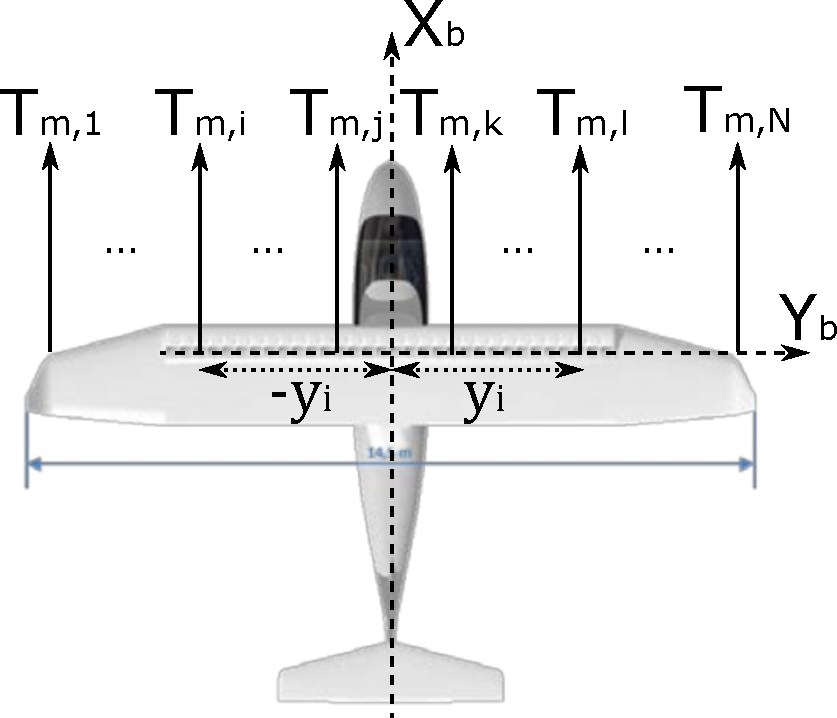
\includegraphics[width=.6\textwidth]{AmpereTop}
	\caption{Illustration of thrust distribution.} Point forces are considered symmetrically placed along the wing. Unlike the configuration of Ampere \cite{Ampere_concept}, equal repartition of engine from root to wing-tip is assumed. \label{fig:AmpereTop}
\end{figure}

Where $T_{x,i}$ and $y_i$ are respectively the thrust force and distance between the body X axis and the i$^{\text{th}}$ motor. 
Our study has previously been limited to propulsive system based on electric engine running propellers. For aircraft equipped with a propeller or a fan, a common thrust model can be \cite{SachsElectricPerf}:
\begin{equation}
	T=PV^{-1} \eta_p \frac{\rho}{\rho_0} \delta x \label{Eq:oldThrustModel}
\end{equation}
Where P is the engine power at sea level, V is the flight velocity, $\eta_p$ is the propeller or fan efficiency, $\rho$ the air density and $\delta_x$ the throttle command. Equation (\ref{Eq:oldThrustModel}) models the loss of power of air breathing engines with variation of air density. Electric motors on the contrary, do not suffer from rarefaction of air as turbomachines, such that we may concider the following thrust model for computing $T_{x,i}$ \cite{SachsElectricPerf}:
\begin{equation}
	T_{x,i}=\frac{P_E}{N}V^{-1}\eta_m\eta_p \delta_{x,i}
\end{equation}
With $P_E$ being the total electrical power available from the line, $N$ being the total number of engine, $\eta_m$ and $\eta_p$ respectively the engine and propeller efficiency (both concidered constant). Hence, we concider that the power is equally divided between each engine. Finally, $\delta_{x,i}$ is the throttle command of each engine and is added to the control input vector : $\textbf{u}=[\delta_a , \delta_e , \delta_R , \delta_{x,1} , \dots , \delta_{x,N}]$. The number of input becomes : $n_u=N_m+3$.

One may argue that electric propulsion will be impacted by altitude anyway. It is true in many aspects, for example:
\begin{itemize}
	\item With increasing altitude cooling of electric engine and power electronics can become more difficult
	\item Maximum rated voltage of conductors decreases with altitude due to Corona effect \cite{WiringSpace}
	\item Finally, in the case of series hybrid or turbo-electric propulsion, the turbo-machine producing the electric power remains sensible to air rarefaction.
\end{itemize}

These limitations are either due to technological locks that can be overcome with increasing interest in electric propulsion or associated with a level of details outside the scope of our study. For these reasons, we will keep the assumption that engine power is constant with altitude.

\subsection{Finding the trim position by optimization}

Similarly to what is done in \cite{GomanAttainableEqui}, a set of additional constraints $N_c$ can now be defined to condition the problem such that only one possible solution exists. The number of variables to determine ($n_x+n_u+n_p$) must equal the number of equations and constraints $N_e+N_c$.
In this case, considering that the number of engine varies, the number of additional constraints to define is given by:
\begin{align}
N_c=&n_x+n_u+n_p-N_e\\
N_c=&N_m+3
\end{align}

In the case where differential thrust is not used, the additional input is $N_m=1$, representing forward thrust or throttle level, and one must fix $N_c=4$ additional constraints, similarly as in \cite{GomanAttainableEqui}. These additional constraints are added to determine the flight condition, typically fixing the following variables: $[V,\beta,\gamma,\Omega]$. With differential propulsion, the minimum number of additional input is $N_m=2$ with two engines. Consequently, the problem becomes quickly overdetermined. An infinite number of equilibrium points can exist. This can be pictured by the different possible combination of throttle level and rudder action to satisfy a certain thrust and yaw moment.

For overdetermined problems, it is common to use optimization methods to find a satisfying solution \cite{OppeinheimerControlAllocation}. Two options are possible: one may define the input vector as $\mathbf{u}=[\delta_a,\delta_e,\delta_n, \delta_x]$ with $\delta_n$ being the total yaw moment input and $\delta_x$ the total thrust force such that the equilibrium problem is well conditioned and then use an optimization method to find the $\delta_R$ and $\delta_{x,i}$. Or one could run the optimization on the complete set of variables. We selected the second option for this study. This is motivated by the will of maintaining a tight coupling between flight dynamics and differential thrust.

It should be stressed that the first option leaves room for development of 
\begin{itemize}
	\item Generic control and allocation laws
	\item Optimal control
	\item Optimisation of design
\end{itemize}

These aspects will be the object of future studies.

Without loss of generality, additional higher and lower bounds are added on control inputs, angle of attack and bank angle depending on the flight phase. For example, the bank angle is limited to $\pm5\degree$ when studying engine failure at take off as stated by flight regulation \cite{CS25}. These bounds are resumed in table \ref{tab:Bonds} and are in part, dependent on the aircraft selected for the study.

The following variables are chosen to imposed the flight conditions $[V,\beta,\gamma,\Omega]$. The objective function to minimize is defined as the power required to maintain equilibrium. Such an objective function makes sense in the point of view of the designer who will look for minimizing the power to install on the aircraft. Finally, to simulate engine failure we simple add a constraint on the throttle level of the corresponding engines.

The problem hence writes:
\begin{align}
\underset{\tilde{x}}{min} & \: \:\sum_{i=1}^{N} T_{x,i} V\\
\text{With:}\qquad \tilde{x}&=[\alpha, p, q, r, \phi, \theta, \delta_a, \delta_e, \delta_R, \delta_{x,1}, \dots, \delta_{x,N}]\\
\text{Subjected to: }&\notag \\
\begin{pmatrix}
0 \\
-mV(p\sin\alpha - r\cos\alpha)\\
mV\left[\sin\beta (p\cos\alpha + r\sin\alpha) - q\cos\beta\right]
\end{pmatrix}
= & mg
\begin{pmatrix}
-\sin\gamma\\
\cos\gamma \sin\mu\\
\cos\gamma \cos\mu	
\end{pmatrix}
+ \frac{1}{2} \rho S V^2
\begin{pmatrix}
-C_d\\
C_Y\\
-C_L
\end{pmatrix}
+ \mathbf{H_{ab}} 
\begin{pmatrix}
\sum_{i=1}^{N} T_{x,i}\\
0\\
0
\end{pmatrix} \\
0 =& \frac{1}{2} \rho S V^2 l
\begin{pmatrix}
C_l\\
C_m\\
C_n
\end{pmatrix}
+
\begin{pmatrix}
0\\
0\\
\sum_{i=1}^{N} T_{x,i} y_i
\end{pmatrix} -
\begin{pmatrix}
p\\
q\\
r
\end{pmatrix}
\times \textbf{I}
\begin{pmatrix}
p\\
q\\
r
\end{pmatrix}\\
0= & p + q\sin\phi \tan\theta + r \cos\phi \tan\theta\\
0= & q\cos\phi -r\sin \phi\\
\Omega = & \left( q \sin \phi + r \cos \phi \right) \sec \theta \\
\sin \gamma = & \cos\alpha\cos\beta\sin\theta - \sin\beta\sin\phi\cos\theta - \sin\alpha\cos\beta\cos\phi\cos\theta\\
0 = & \delta_{x,1}\\
\vdots\notag\\
0 = & \delta_{x,j}
\end{align}

The problem being now defined, the next section will treat the constitution of the aerodynamic database to compute the aerodynamic coefficients in function of VT area as well as flight phase.

\begin{table}[hbt!]
	\caption{\label{tab:Bonds} Additional bounds depending on flight phase}
	\centering
	\begin{tabular}{l|c|c|c}
		Flight phase & $V<71 m.s^{-1}$& $V>71 m.s^{-1}$ & Engine failure\\
		\hline
		$\alpha (\degree)$ & $-2\leq\alpha\leq 10$ & $-2\leq\alpha\leq 15$ & (-) \\
		$\phi (\degree)$ & $\pm 30$ & $\pm 30$ & $\pm 5$\\ 
		$\theta (\degree)$ & $\pm 30$ & $\pm 30$& $\pm 30$\\
		$\delta_a(\degree)$ & $\pm 20$& $\pm 20$& $\pm 20$\\
		$\delta_e(\degree)$ & $\pm 20$ & $\pm 20$ & $\pm 20$\\
		$\delta_R(\degree)$ & $\pm 25$ & $\pm 25$ & $\pm 25$\\
		$\delta_{x,i}$ & $0< \delta_{x,i} \leq 1$ & $0< \delta_{x,i} \leq 1$ & $0< \delta_{x,i} \leq 1$ \\
	\end{tabular}
\end{table}



\clearpage

\section{Aerodynamic database}
In this section, it is explained how the aerodynamic database was obtained to study the effect of varying the vertical tail surface area. Assumptions are re-called to put the focus only on relaxed lateral stability.

\subsection{Reference Aircraft}
The method developed up to now is generic and could be used with any aircraft given the corresponding aerodynamic characteristics. To study the differences between a traditional configuration and a DEP aircraft, a baseline aircraft representing the class of aircraft most probable for electric propulsion and distributed propulsion has to be selected. Commuters aircraft are often cited as the next big step in developing electric airplanes since most of their mission are within the limits of electric propulsion in terms of endurance \cite{MisconceptionMoore} \cite{StucklMethodsDesignElectriProp}. These aircrafts usually are equipped with turboprop engine and fly at subsonic velocity. A good representative of this class of aircraft is the ATR72 which details are reported in table~\ref{tab:nominalset}.

\begin{table}[hbt!]
	\caption{\label{tab:nominalset} ATR 72 general details \cite{ATRFAAtypecertificate}, \cite{JanesAircraft}}
	\centering
	\begin{tabular}{l|c}
		Variables & Value\\
		\hline
		Wingspan & 27 m\\
		Wing surface area & 61 m$^2$\\ 
		VT surface area & $12$ $\textrm{m}^2$\\
		Engine level arm & 4.1 m\\
		Masse & 21500 Kg\\
		Total available power & 4 000 KW\\
		Stall velocity $V_s$ & 56 m/s\\
	\end{tabular}
\end{table}

So far, special care was given to keep the analysis as generic as possible to be able to compare flight qualities of different aircraft configurations. Following the same philosophy it is assumed no change in the geometry, mass or power available of the reference ATR72 between the baseline configuration and the electric propelled one.

The only feature allowed to change is the vertical tail which will be reduced so as to obtain relaxed lateral stability or a lightly unstable aircraft. Consequently, we will analyse a weakly unconventional aircraft configuration.

\subsection{Building the Aerodynamic Database}
For unconventional configurations, it is necessary to carefully select the method with which one can establish the aerodynamic database. As Chudoba explains in \cite{ChudobaUnconventionalConf}, the means of calculating aerodynamic characteristics can be organized in three categories summurised in Table~\ref{tab:aeroAnalysis}.
\begin{table}[hbt!]
	\caption{\label{tab:aeroAnalysis} Methods for Aerodynamic Analysis \cite{Chudoba_generic_method}}
	\centering
	\begin{tabular}{l|c}
		Category & Example of methods\\
		\hline
		Analytical & Lifting Line, Swept Wing Theory, ...\\
		Empirical, semi-empirical & DATCOM, ESDU, ...\\ 
		Numerical & Vortex Lattice Method, Panel Method, CFD, ...\\
	\end{tabular}
\end{table}

Both analytical and empirical/semi-empirical methods are built on experiences and analysis of conventional configurations. Therefore there can hardly be concidered as generic methods. Numerical methods offer different level of fidelity allowing to capture the specificity of unconventional design. For preliminary designs, VLM or Panel Method, both linear technics, are often prefered over CFD for their favorable precision relative to computational cost.

Although our configuration is only weakly unconventional, capturing the effect of geometrical changes in VT isn't something that analytical of empirical/semi-empirical methods can do because of the important influence of other aircraft components on the flow impacting the VT. This has been demonstrated by Nicolosi in \cite{NicolosiInvestigationVertical}, where his research team investigated the differences obtained between DATCOM, ESDU estimation technics and CFD methods complemented with wind tunnel experiments.

The main contributors to flow perturbation impacting the VT are the fuselage and the horizontal tail which are acting as end plates, reducing the downwash at the root and tip of the vertical tail. 

Using numerous CFD simulations complemented with wind tunnel test on a generic commuter aircraft model, Nicolosi and his research team could establish a new semi-empirical method called VeDSC. This method focuses on predicting the VT efficiency as a function of VT geometry and aircraft components. The main assumption is the fact that contribution of each components of the aircraft on lateral coefficients; $C_{Y}$, $C_{p}$, $C_{r}$ $\equiv C_{\textrm{lat}}$, can be decoupled in the following way:
\begin{eqnarray}
C_{\textrm{lat}_\beta} = C_{\textrm{lat},F_\beta} + C_{\textrm{lat},W_\beta} + C_{\textrm{lat},v_\beta}
\end{eqnarray}
Where it is assumed that the contribution of the VT, $C_{\textrm{lat},v_\beta}$ is influenced by the fuselage, wing and horizontal tail but does not influence the other coefficients $C_{lat,F_\beta}$ and $C_{lat,W_\beta}$.
The VeDSC method furnishes a way to estimate the coefficient $C_{\textrm{lat},v_\beta}$ through a reformulation of the VT lift slope coefficient defined as follow:
\begin{equation}
a_v=K_F K_W K_H C_{L,v_\beta}
\end{equation}
Where $C_{L,v_\beta}$ is the lift slope of a swept wing determined using Diederich formula for swept wing \cite{DiederichPlanformParameter}. $K_F$, $K_W$ and $K_H$ are corrective coefficients taking into account respectively the fuselage, wing and horizontal tail effects. The reader is refered to \cite{NicolosiVTDesignReview} and \cite{NicolosiDirectionalStabilityReviewofEmpiricalMethod} for the complete formulation of these parameters.

The VT contribution to lateral coefficients is then calculated using formulas given by Etkin \cite{Etkin}:
\begin{align}
&C_{Y_\beta} = a_v\frac{S_v}{S}\left( 1-\frac{\partial \sigma}{\partial \beta}\right) 
&&C_{l_\beta} =-a_v\frac{S_v z_v}{S b}\left( 1-\frac{\partial \sigma}{\partial \beta}\right) 
&&&C_{n_\beta} = a_v V_v\left( 1-\frac{\partial \sigma}{\partial \beta}\right)\\
&C_{Y_p} = -a_v\frac{S_v}{S}\left(2\frac{z_v}{b}-\frac{\partial \sigma}{\partial \hat{p}}\right) && \qquad &&&C_{n_p}= a_v V_v\left(2\frac{z_v}{b}-\frac{\partial \sigma}{\partial \hat{p}}\right)\\
&C_{Y_r} = a_v\frac{S_v}{S}\left( 2\frac{l_F}{b}+\frac{\partial \sigma}{\partial \hat{r}}\right)  &&C_{l_r} =a_v\frac{S_v z_v}{S b}\left( 2\frac{l_F}{b}+\frac{\partial \sigma}{\partial \hat{r}}\right) &&&C_{n_r} = -a_v V_v\left( 2\frac{l_v}{b}-\frac{\partial \sigma}{\partial \hat{r}}\right)
\end{align}

This semi-empirical methods required hundreds of CFD simulations to explore a wide variety of parameter changes. Variation and validity intervals of some parameters of interest are shown in Table~\ref{tab:VeDSCParam}. The method could be extrapolated to VT of aspect ratio from 0.5 to 4 since the Diederich formula is valid for these values however the correcting terms would be out of interpolation range.



Overall the VeDSC method turns to be an adequate semi-empirical method to be used with our reference aircraft. In addition, having a formula to estimate the VT efficiency instead of running a VLM is an important time saving aspect.

In order to establish our aerodynamic database, we modeled the ATR72 without its VT into VSPaero using publicly available data essentially from \cite{JanesAircraft}. The VLM included in VSPaero is then used to establish the longitudinal coefficients and contribution to the lateral coefficients. The contribution of the fuselage and wing to lateral coefficients has been found to be adequatly estimated by the VLM. It is then complemented with the VeDSC method to quickly and accurately account for the changes in VT geometry. This renders the database extremely agile since we only need to run VLM simulations once.

\begin{figure}[hbt!]
	\centering
	\begin{subfigure}[b]{0.33\textwidth}
		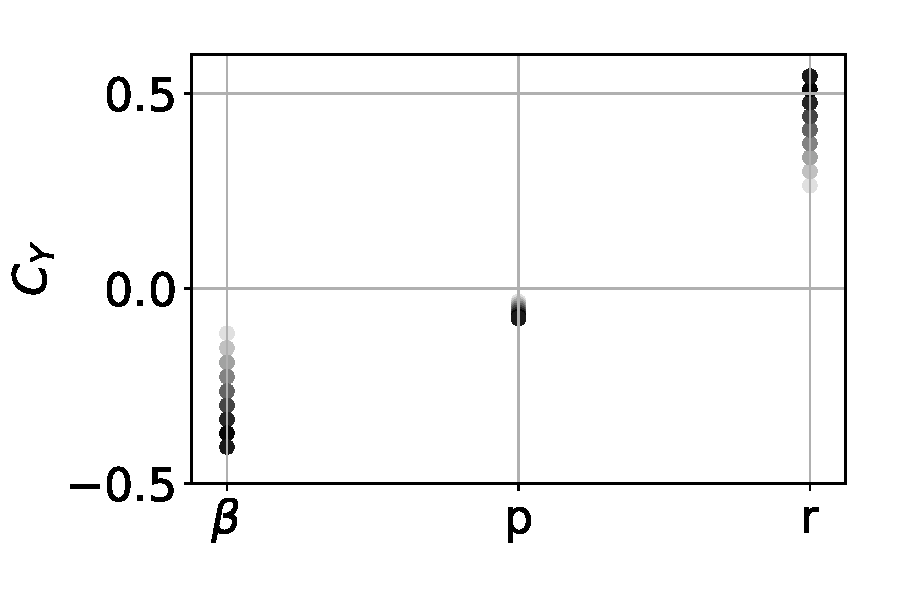
\includegraphics[width=1.0\textwidth]{CyCstAR}
		\caption{All derivatives per rad}
		\label{fig:CyCstAR}
	\end{subfigure}
	%add desired spacing between images, e. g. ~, \quad, \qquad, \hfill etc. 
	%(or a blank line to force the subfigure onto a new line)
	\begin{subfigure}[b]{0.33\textwidth}
		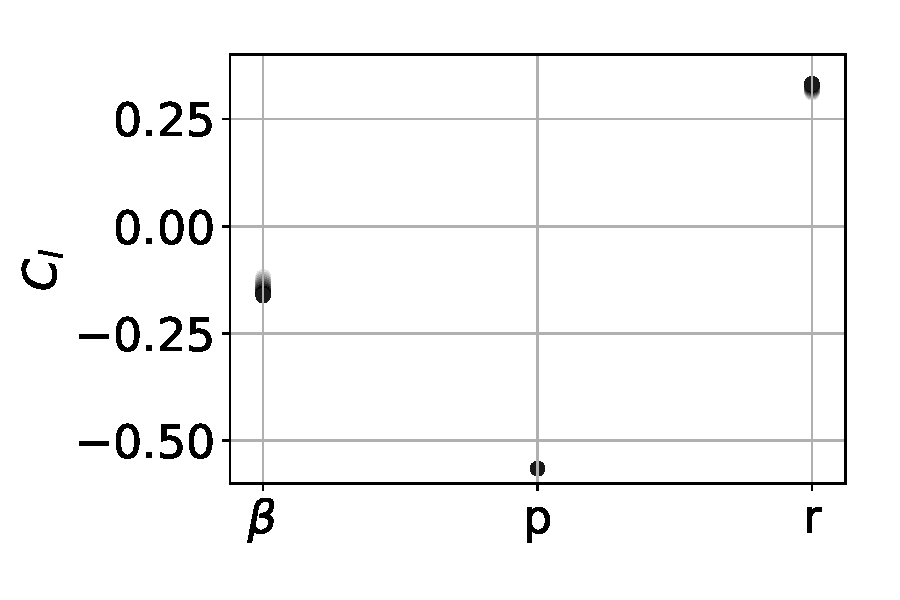
\includegraphics[width=1.0\textwidth]{ClCstAR}
		\caption{All derivatives per rad}
		\label{fig:ClCstAR}
	\end{subfigure}
	%add desired spacing between images, e. g. ~, \quad, \qquad, \hfill etc. 
	%(or a blank line to force the subfigure onto a new line)
	\begin{subfigure}[b]{0.33\textwidth}
		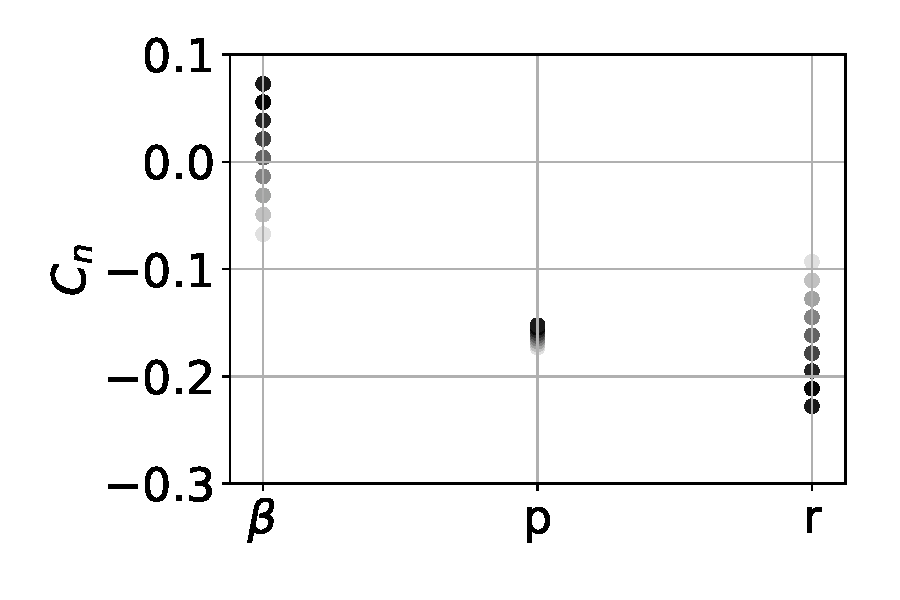
\includegraphics[width=1.0\textwidth]{CnCstAR}
		\caption{All derivatives per rad}
		\label{fig:CnCstAR}
	\end{subfigure}
	\caption{Evolution of lateral coefficients of total aircraft with variation of VT area for constant AR.} Whitest marker represents $S_v=0.1S_{v,0}$, darkest represents $S_v=S_{v,0}$, per step of $0.1S_{v,0}$.\label{fig:cstAR}
\end{figure}

To explore the flight performances in the whole flight envelop, it has been chosen to use a database in function of mach number as only flight parameter. For low speed flight, when the flaps are used, the parameters are assumed to be constant. Then, they vary with the mach number. The evolution of some coefficients with Mach number is illustrated in Fig~\ref{fig:MachVariation}. The Mach number 0.2 taken at see level represents the minimum flight velocity of the ATR72 without flaps.

\begin{figure}[hbt!]
	\centering
	\begin{subfigure}[b]{0.33\textwidth}
		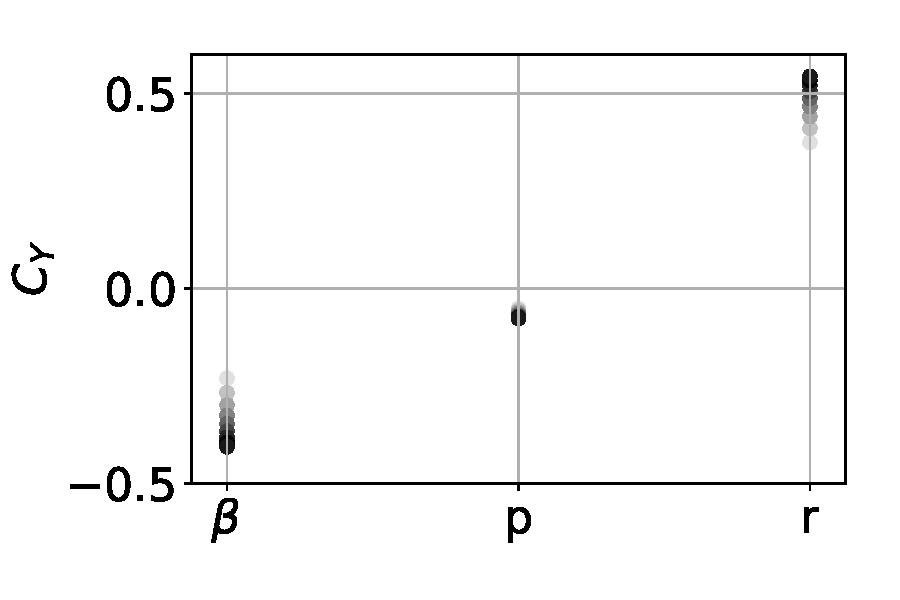
\includegraphics[width=1.0\textwidth]{CyCstSpan}
		\caption{All derivatives per rad}
		\label{fig:CyCstSpan}
	\end{subfigure}
	%add desired spacing between images, e. g. ~, \quad, \qquad, \hfill etc. 
	%(or a blank line to force the subfigure onto a new line)
	\begin{subfigure}[b]{0.33\textwidth}
		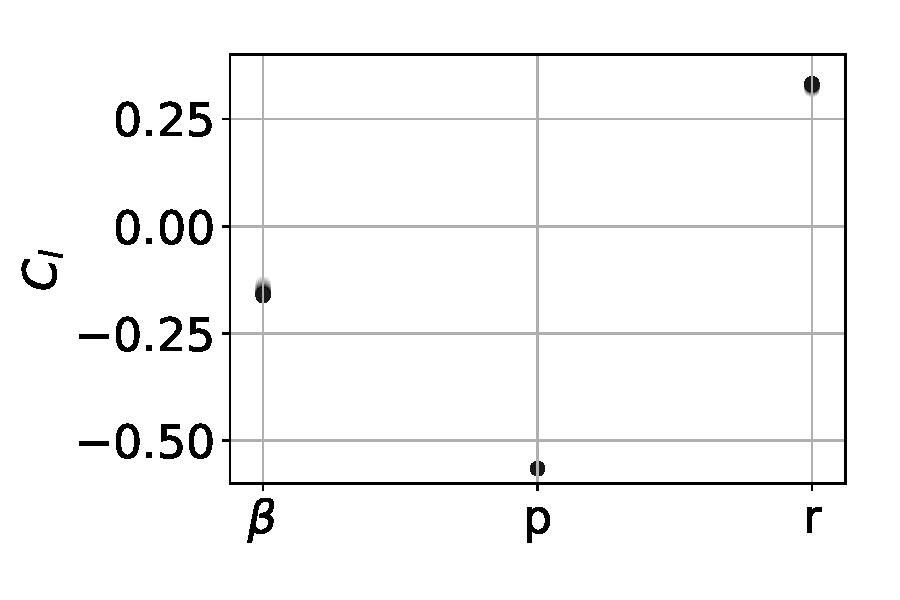
\includegraphics[width=\textwidth]{ClCstSpan}
		\caption{All derivatives per rad}
		\label{fig:ClCstSpan}
	\end{subfigure}
	%add desired spacing between images, e. g. ~, \quad, \qquad, \hfill etc. 
	%(or a blank line to force the subfigure onto a new line)
	\begin{subfigure}[b]{0.33\textwidth}
		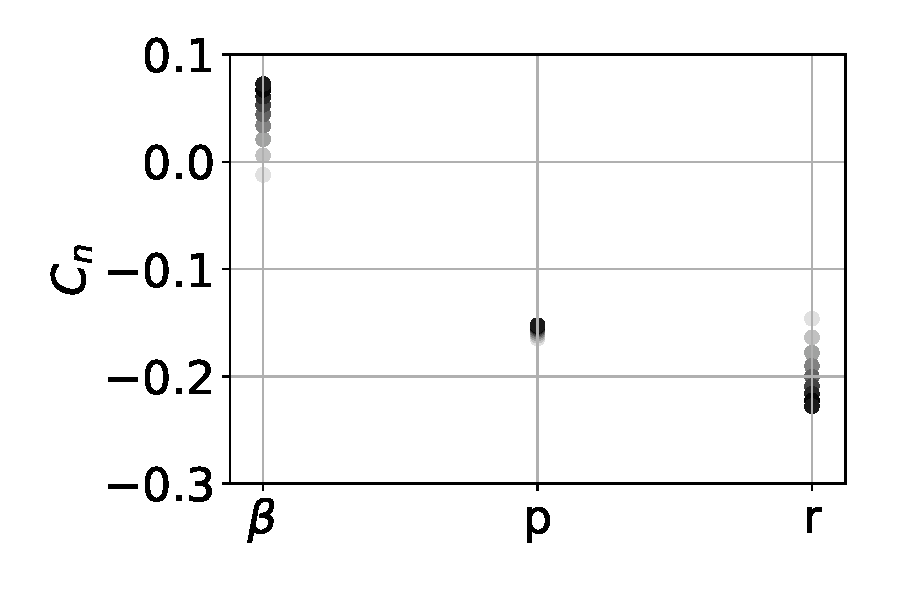
\includegraphics[width=1.0\textwidth]{CnCstSpan}
		\caption{All derivatives per rad}
		\label{fig:CnCstSpan}
	\end{subfigure}
	\caption{Evolution of lateral coefficients of total aircraft with variation of VT area for constant span.} Whitest marker represents $S_v=0.3S_{v,0}$, darkest represents $S_v=S_{v,0}$, per step of $0.1S_{v,0}$ The interval of AR swept is $[1.56,5.21]$\label{fig:cstSpan}
\end{figure}


\begin{figure}[hbt]
	\centering
	\begin{subfigure}[b]{0.49\textwidth}
		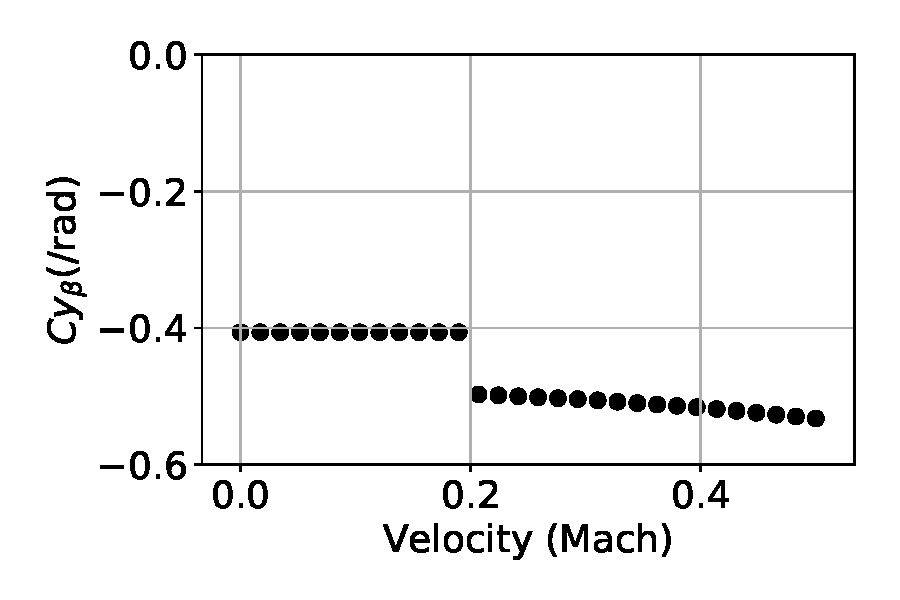
\includegraphics[width=0.8\textwidth]{CybetaMachChange}
		\caption{}
		\label{fig:CybetaMachChange}
	\end{subfigure}
	%add desired spacing between images, e. g. ~, \quad, \qquad, \hfill etc. 
	%(or a blank line to force the subfigure onto a new line)
	\begin{subfigure}[b]{0.49\textwidth}
		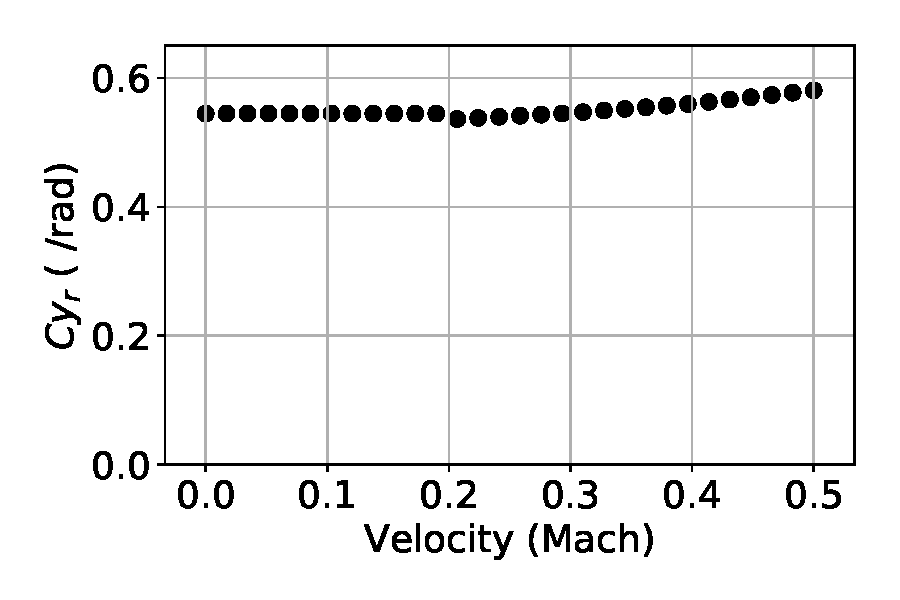
\includegraphics[width=0.8\textwidth]{CyrMachChange}
		\caption{}
		\label{fig:CyrMachChange}
	\end{subfigure}
	\\
	%add desired spacing between images, e. g. ~, \quad, \qquad, \hfill etc. 
	%(or a blank line to force the subfigure onto a new line)
	\begin{subfigure}[b]{0.49\textwidth}
		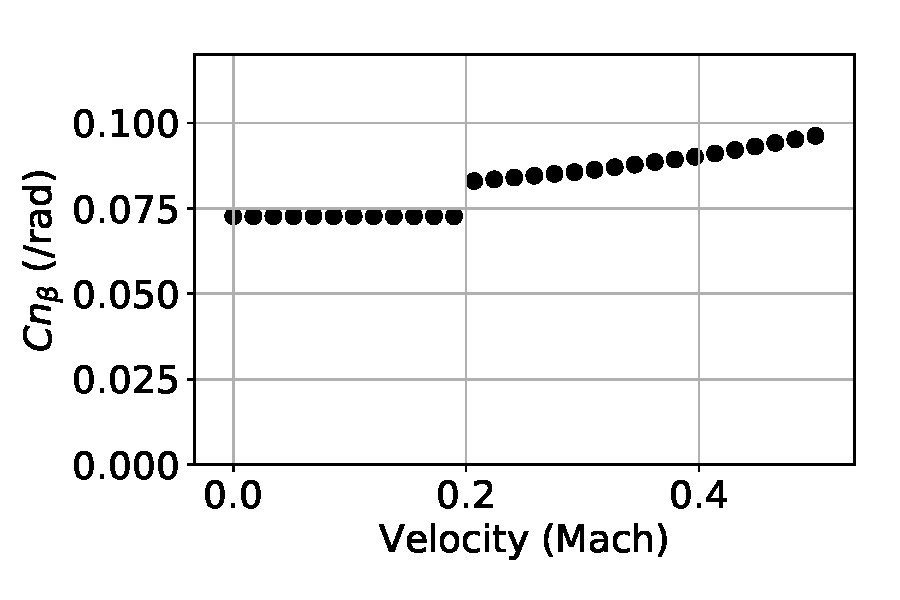
\includegraphics[width=0.8\textwidth]{CnbetaMachChange}
		\caption{}
		\label{fig:CnbetaMachChange}
	\end{subfigure}
	\begin{subfigure}[b]{0.49\textwidth}
		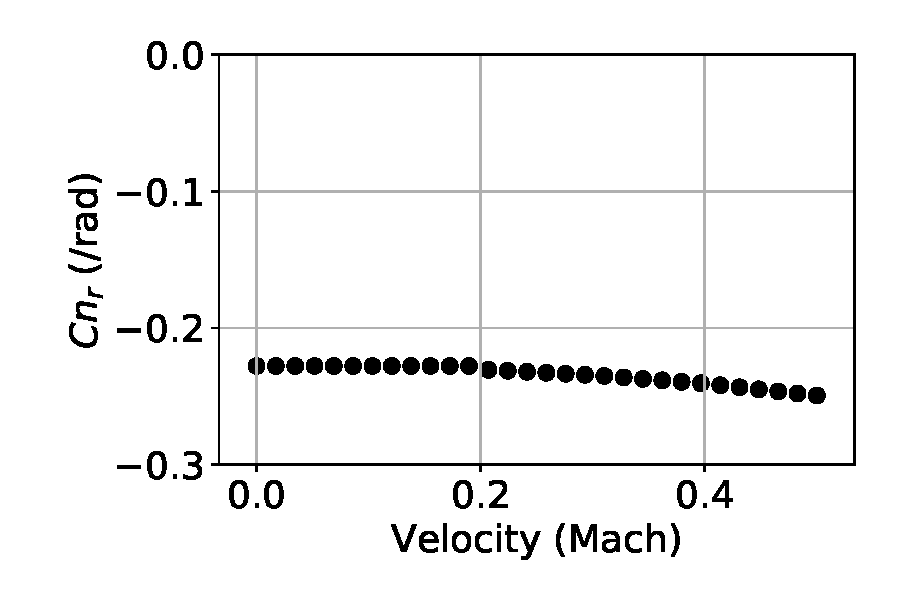
\includegraphics[width=0.8\textwidth]{CnrMachChange}
		\caption{}
		\label{fig:CnrMachChange}
	\end{subfigure}
	\caption{Evolution of lateral coefficients of total aircraft with Mach number.}\label{fig:MachVariation}
\end{figure}

Finally, two ways of modifying the vertical tail are available. The first is the change of surface area while maintaining the aspect ratio constant. This gives linearly varying coefficients as it can be seen in fig~\ref{fig:cstAR}. The second comes from the fact that one may want to keep the horizontal tail high to avoid the slipstream of the propellers, hence the surface should be reduced without modifying the span. In turn the aspect ratio is increased up to reasonnable values to limit extrapolation as shown in fig~\ref{fig:cstSpan}. This variation induces non linear variation of the coefficient and may be find useful for flight qualities.

\begin{table}[hbt]
	\caption{\label{tab:VeDSCParam} A few parameter ranges on which VeDSC has been constructed. From \cite{NicolosiNewApproach}} 
	\centering
	\begin{tabular}{l|l|c}
		Parameters & Description & Range\\
		\hline
		$A_v$ & VT aspect ratio & $\left[1,2\right]$\\
		$A_W$ & Wing aspect ratio & $\left[6,16\right]$\\
		$z_W$ & Wing vertical position, relative to fuselage centerline & $\left[-1,1\right]$ \\
		$z_H$ & Horizontal Tail Vertical Position, relative to VT span & $\left[0,1\right]$\\
		$\frac{S_H}{S_v}$ & Relative Horizontal tail surface area & $\left[0.5,2\right]$
	\end{tabular}
\end{table}

\clearpage

\section{Results}

Voici des examples des cartes d'équilibres que je peux générer avec l'outil. Tout les résultats sont générés pour un cas de panne moteur(s) au décollage en concervant un angle de montée de 2°. (Les conditions seront résumés dans un tableau pour la version final)

Mon idée est de faire passer le plus d'information avec le moins de graphs possible. Je me concentrerai sur la phase de décollage avec des cartes en vitesse-versus-dérapage. En plus j'ajouterai un example de répartition de poussée et d'attitude de l'avion typique pour une DEP avec panne moteur. Qu'est-ce que vous en penser?

\begin{figure}[hbt!]
	\centering
	\begin{subfigure}{0.49\textwidth}
		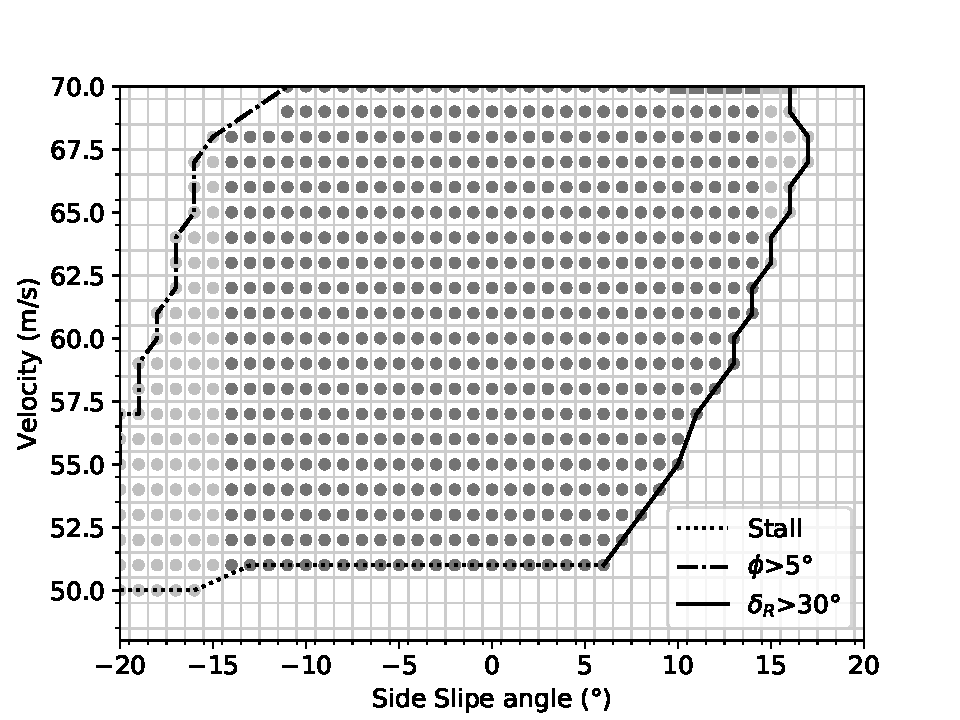
\includegraphics[width=0.95\textwidth]{originalMapBetaVelfin1Eng3RudFalse}
		\caption{Original ATR72 with one engine failure.}
		\label{fig:originalfin1_3engine}
	\end{subfigure}
	\begin{subfigure}{0.49\textwidth}
		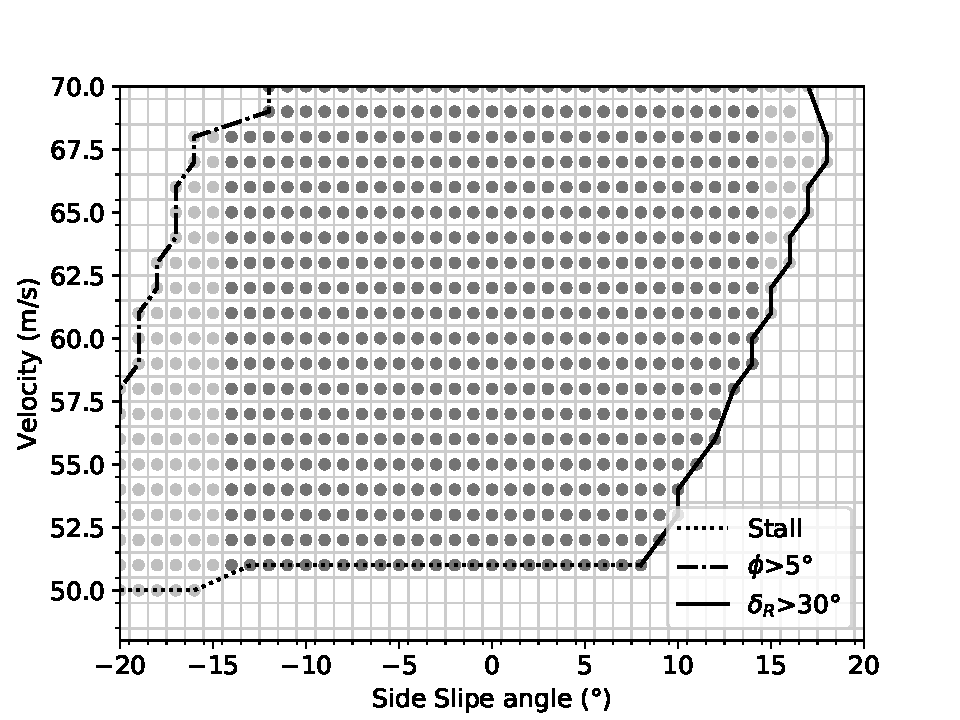
\includegraphics[width=0.95\textwidth]{originalMapBetaVelfin1Eng15RudFalse}
		\caption{ATR with 12 engines, three inoperatives.}
		\label{fig:originalfin1_15engine}
	\end{subfigure}
	\caption{Original ATR with \ref{fig:originalfin1_3engine} twin engine, one inoperational and \ref{fig:originalfin1_15engine} twelve engines, three inoperationals. Only the rudder is used to compensate the yawing moment.}
\end{figure}

\begin{figure}
	\begin{subfigure}{0.49\textwidth}
		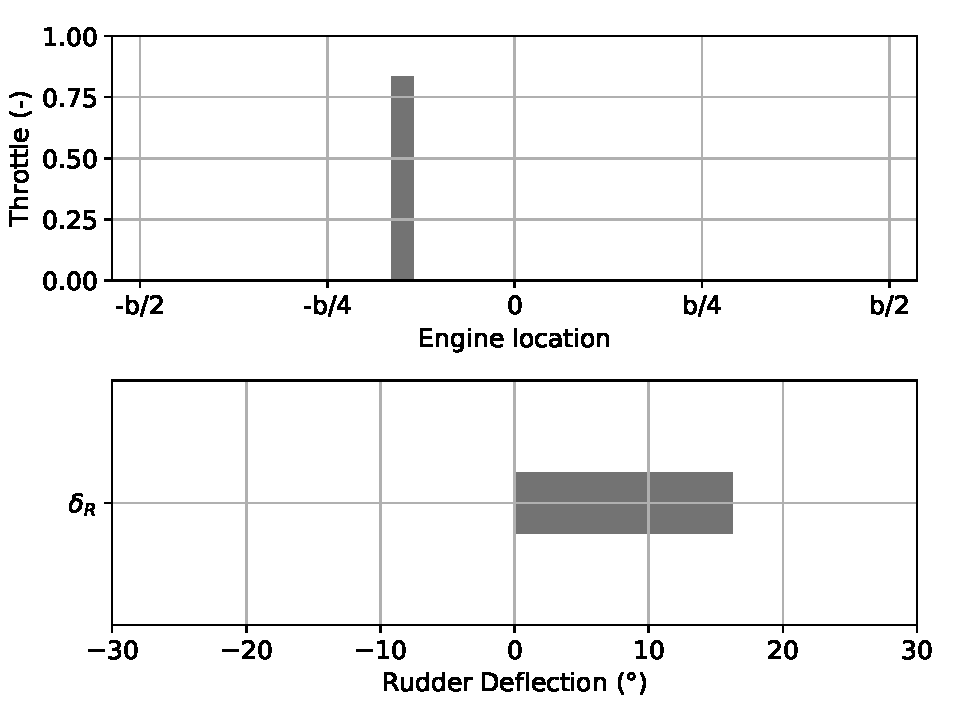
\includegraphics[width=0.95\textwidth]{Defloriginalfin1Eng3RudFalse}
		\caption{Original ATR72 with one engine failure.}
		\label{fig:Defloriginalfin1_3engine}
	\end{subfigure}
	\begin{subfigure}{0.49\textwidth}
		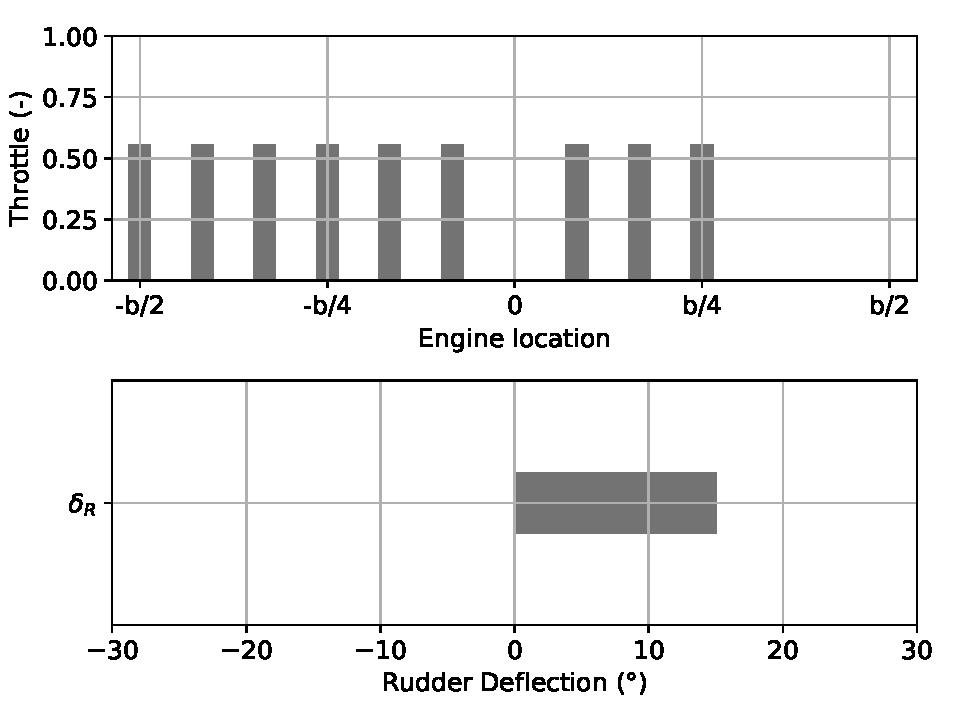
\includegraphics[width=0.95\textwidth]{Defloriginalfin1Eng15RudFalse}
		\caption{Original ATR with twelve engines, three inoperatives.}
		\label{fig:Defloriginalfin1_15engine}
	\end{subfigure}
	\caption{Throttle level and rudder deflection for trim at V=60m/s, $\beta=0$}
\end{figure}

\begin{figure}[hbt!]
		\centering
		\begin{subfigure}{0.49\textwidth}
			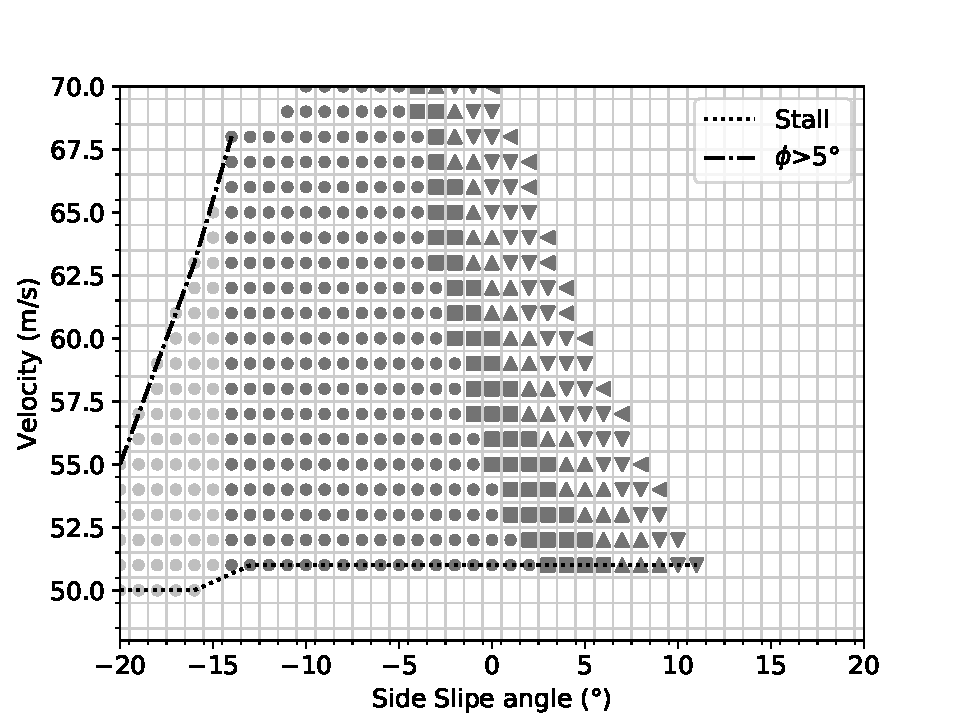
\includegraphics[width=0.95\textwidth]{DEPoriginalMapBetaVelfin1Eng15RudTrue}
			\caption{Flight envelop, ATR with 12 engines, three inoperatives.}
			\label{fig:DEPoriginalfin1_15engine}
		\end{subfigure}
		\begin{subfigure}{0.49\textwidth}
			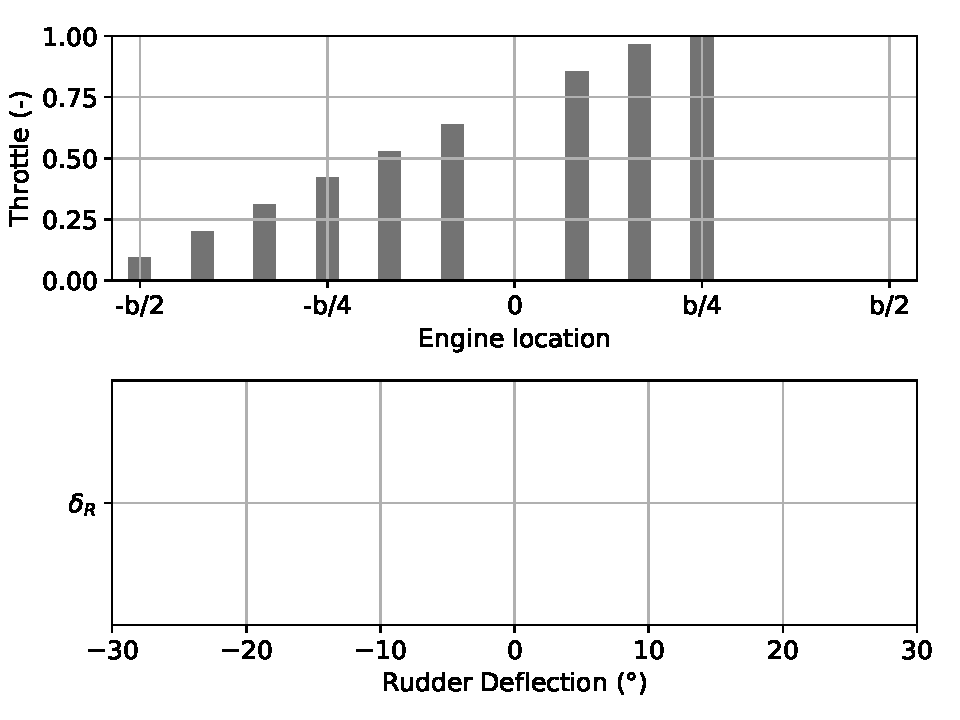
\includegraphics[width=0.95\textwidth]{DeflDEPoriginalfin1Eng15RudTrue}
			\caption{Throttle level and Rudder deflection at 60m/s and $\beta=0\degree$, ATR72 with 12 engines, three inoperatives.}
			\label{fig:DeflDEPoriginalfin1_15Eng}
		\end{subfigure}
		\caption{ATR72 using only differential thrust. Circles indicate an equilibrium point, rectangle indicate an equilibrium with at least one engine at saturation (full throttle)}
\end{figure}

\begin{figure}[hbt!]
	\centering
	\begin{subfigure}{0.49\textwidth}
		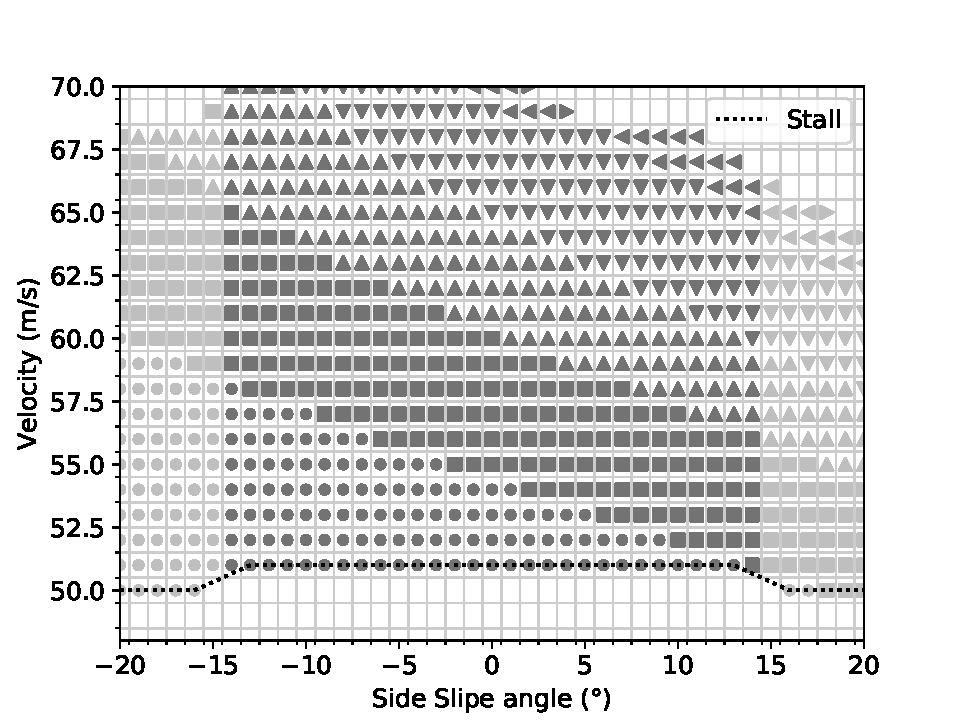
\includegraphics[width=0.95\textwidth]{DEPoriginalMapBetaVelfin07Eng15RudTrue}
		\caption{ATR with 12 engines, three inoperatives and $S_v=0.7S_{v_0}$. Rudder not used. Circles indicate an equilibrium point, rectangle indicate an equilibrium with at least one engine at saturation (full throttle)}
		\label{fig:DEPoriginalfin07_15engine}
	\end{subfigure}
	\begin{subfigure}{0.49\textwidth}
		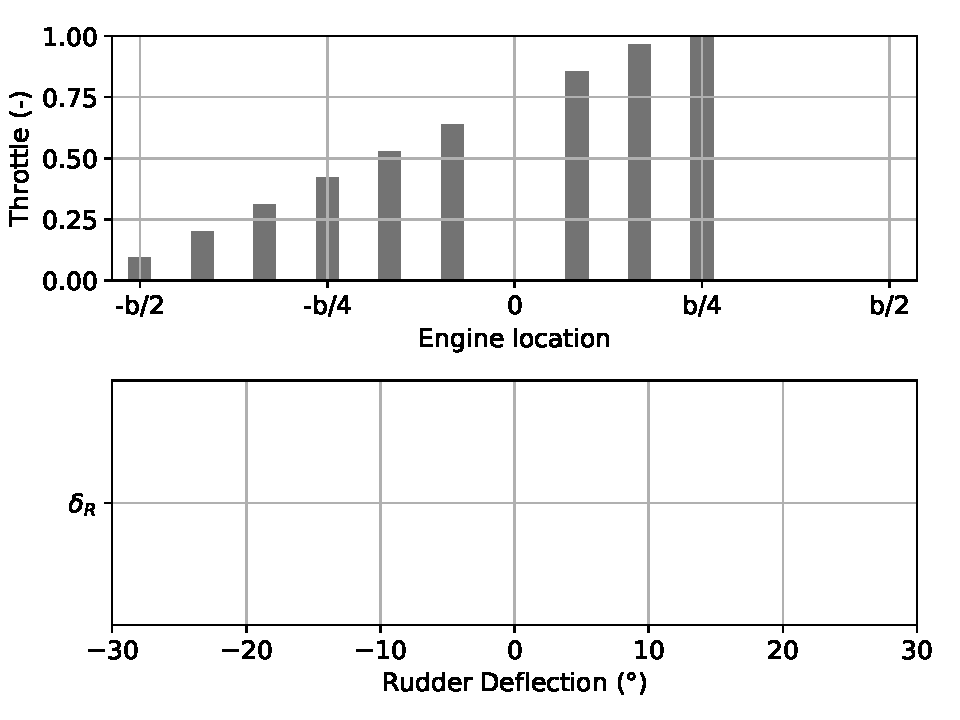
\includegraphics[width=0.95\textwidth]{DeflDEPoriginalfin07Eng15RudTrue}
		\caption{Throttle level and Rudder deflection at 60m/s and $\beta=0\degree$, ATR72 with 12 engines, three inoperatives, $S_v=0.7S_{v_0}$.}
		\label{fig:DeflDEPoriginalfin07_15Eng}
	\end{subfigure}
\end{figure}

%----- Study Case -----
%One original ATR72 at take off without failed engine next to the same ATR72 at Take off with SEF:
%	Shows that Vmc is found for take off,
%	Show that control is maintained at 1.3Vsr (=15° yaw toward inoperative engine)
%	shows that no equilibrium exists,
%	eventually show the degradation of equilibrium with reduced VT
%	Show the engine saturation at high speed

%Show the same ATR with distributed propulsion:
%	Show input histogramme with and without rudder
%	Show map without rudder and with small rudder
%	Show map with small fin and rudder
%
%At take off means :
%	3% slope for more than 4 engine condition, 
%	2.4 % for twin engine with landing gear retracted (CS.25.121)
%	Not necessarly full power but explore by going higher (in speed mostly)
%	0 altitude
%Maybe replace velocity scale by Vsr, 1.3Vsr etc... as defined by CS

% ATR at 21.5T Vapp=56m/s if it is 1.13Vsr then Vsr=49.55m/s, 1.3Vsr=64.4m/s
% Eventually look at the 20° turns requirement from the certif

%
%Determine 1.3V_{sr} for CS25.147 stating 15° yaw in the direction of the inoperative engine.
%STATE MINIMUM DRAG and 

\clearpage 


\section{Conclusion}
%We are studying the possibility of reducing lateral static stability of an aircraft using Distributed Electric Propulsion and differential thrust. Attention was brought onto the advantages and current difficulties of reducing the area of the fin. Thanks to a new propulsion technology that will be tested in flight in the following years, we suggested that using differential thrust in combination with electric engines is a reliable way to greatly reduced the vertical stabilizer.
%The potential of this idea is studied by looking at static equilibriums in critical phases of engine failure at take off, which is the dimensioning case for vertical stabilizer.
%Preliminary results show sensibility analysis and good performances. Reduction of total installed power seems feasible as well as excellent redundancy depending on total power installed. Following results will include parametric modelisation of the aircraft and aerodynamic simulation tools to better capture the reduction of vertical stabilizer on the aerodynamic coefficients. Dynamic behaviour with basic control law and behaviour at high velocity will also be investigated.

%\clearpage
%\section{Structure}
%
%\section{Introduction}
%\subsection{Aircraft design, stability requirements}
%\begin{itemize}
%	\item Laterale stability is fixed primarily by certification requirements \textbf{cite EASA CS, thèse Feuersanger, sweeping jets others}.
%	\item Name quantities used to qualify performances $V_{mc}$, extreme conditions.
%\end{itemize}
%
%\subsection{Reduction of stability, history}
%\begin{itemize}
%	\item Name aircrafts flying with reduced longitudinal static stability, and name means of stabilization (\textbf{cite abzug}). 
%	\item Introduce the new design schem and CCV domain (\textbf{Find more litterature and aircraft examples})
%\end{itemize}
%
%
%\subsection{Reduction of stability on laterale axis}
%\begin{itemize}
%	\item Name work performed on laterale axis
%	\item Cite the difficulties encountered for this axis due to stability and control requirements in emergency situations. 
%	\item Cite precedent work on reduction of the VT by rendering it more efficient using sweeping jet (\textbf{cite sweeping jets}) both as a mean and potential gains
%	\item cite augmented CCV NASA study
%\end{itemize}
%
%
%\subsection{Differential thrust}
%
%\begin{itemize}
%	\item Introduce electric propelled airplanes and design changes concerning this technology, in particular efficency versus size, possibilities of having distributed engines to take advantages of aerodynamic blowing \textbf{cite NASA, ampere}.
%	\item This study aims at exploring the possibilities offered by such a configuration.
%\end{itemize}
%
%
%\subsection{Structure of the study}
%\begin{itemize}
%	\item What do we aim -> regional transport aircraft which are the first forseen to be manufactured
%	\item How do we contribute -> explore faisability, sensibility parameters such as power to install, configurations and control strategy to the destination of the designer. Ready a brick to include to multi-disciplinary optimization
%	\item Mean -> simulation study, construction of the simulator and design loop with quick and low fidelity aero simulation tools. Control loops tested versus actuation performances (thrust delivered, position of thrust and reaction time).
%\end{itemize}
%
%\section{Preliminary results}
%Based on experimentally determined coefficients of a Beech99 non-linear motion model. Lateral coefficients being artifically reduced proportionally to the surface of the VT.
%\begin{itemize}
%	\item \textbf{Static requirements} from static equilibrium.
%	\item Identification of the problem, over determined system. \textbf{cite overdetermined systems} application of different methodology.
%	\item Dynamic requirements
%\end{itemize}
%
%
%\section{Work remaining}
%Increase fidelity using more elaborated aero tools and a parametric representation of the aircraft in order to determine through simulation aero coefficients of the aircraft with and without VT.
%Complete sensibility analysis.
%Explore the limitations at larger velocity.
%Explore dynamic behaviour and control allocation strategy in linear and non-linear simulations.



\section*{Acknowledgments}
The author would like to thank Mamoun El Oueldrhiri for his support in the exploration of equilibriums with distributed propulsion.

\bibliography{sample}

\end{document}
